\chapter{Afgeleide klasse en objecten in C++}

Bij deze opdracht richten we ons hoe bij OO componenten Overerving en Polymorfisme getest kunnen worden met een debugger.

Deze opdracht bestaat verder uit de deelopdrachten A en B en er moeten 6 screenshots gemaakt worden die op brightspace moeten worden geüpload. Alle deelopdrachten moet je laten aftekenen door de docent.

Er zijn diverse soorten LEDs, zoals in figuur \ref{fig:LEDs} te zien zijn. Deze zijn:
\begin{itemize}
	\item SingleLed: deze LEDs hebben 1 kleur, twee pootjes en worden aan 1 poort op de RockPi aangesloten, zoals de rode, oranje en groene LED. Een voorbeeld wordt weergegeven in figuur \ref{fig:singleLed}
	\item DualLed: deze LEDs hebben 2 mogelijke kleuren, drie pootjes en worden aan 2 poorten (1 per kleur) aan de RockPi verbonden. Een voorbeeld wordt weergegeven in figuur \ref{fig:dualLed}
	\item RGB Led: deze LEDs hebben de kleuren rood, groen en blauw in 1 behuizing en hebben vier pootjes, waarvan 3 worden aangesloten op de poorten (1 per kleur) van de RockPi.De LED met de witte kleur op het practicumboord is een RGB LED. Een voorbeeld van een RGB LED wordt weergegeven in figuur \ref{fig:rgbLed}
\end{itemize}

\begin{figure}[h!]
	\centering
	\begin{subfigure}[b]{0.3\textwidth}
		\centering
		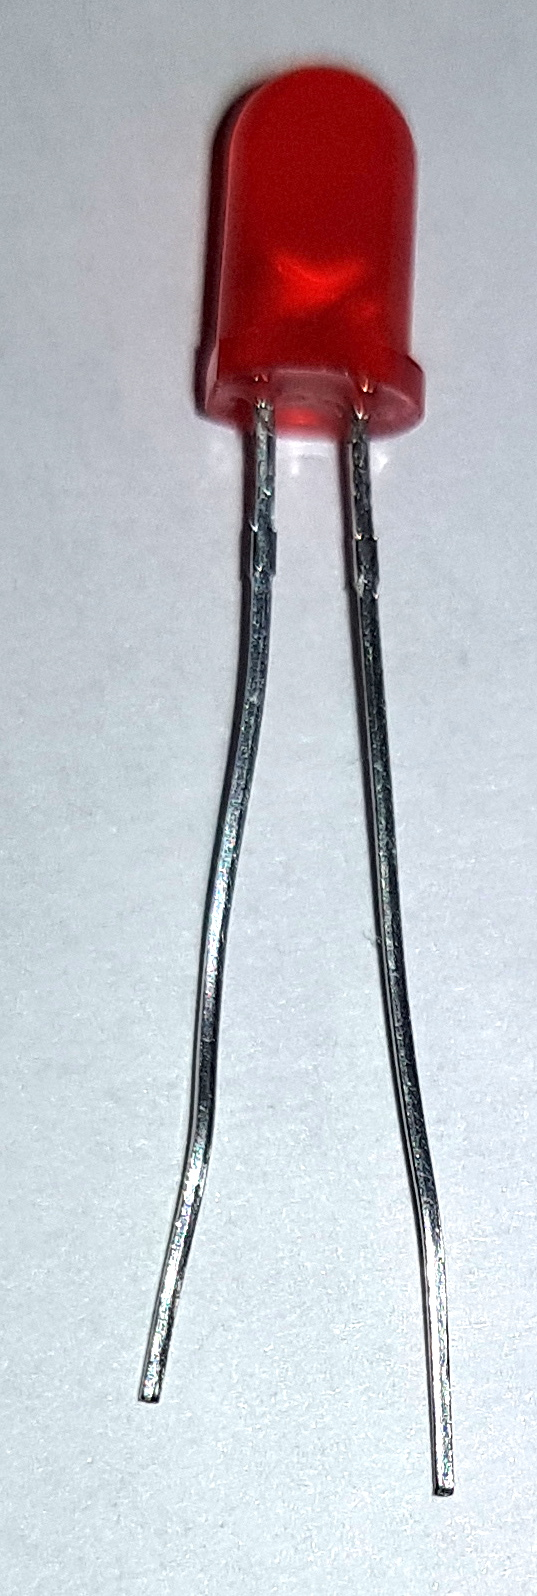
\includegraphics[width=0.7\textwidth,height=3.5cm]{figuren/singleled}
		\caption{een single LED}
		\label{fig:singleLed}
	\end{subfigure}
	\hfill
	\begin{subfigure}[b]{0.3\textwidth}
		\centering
		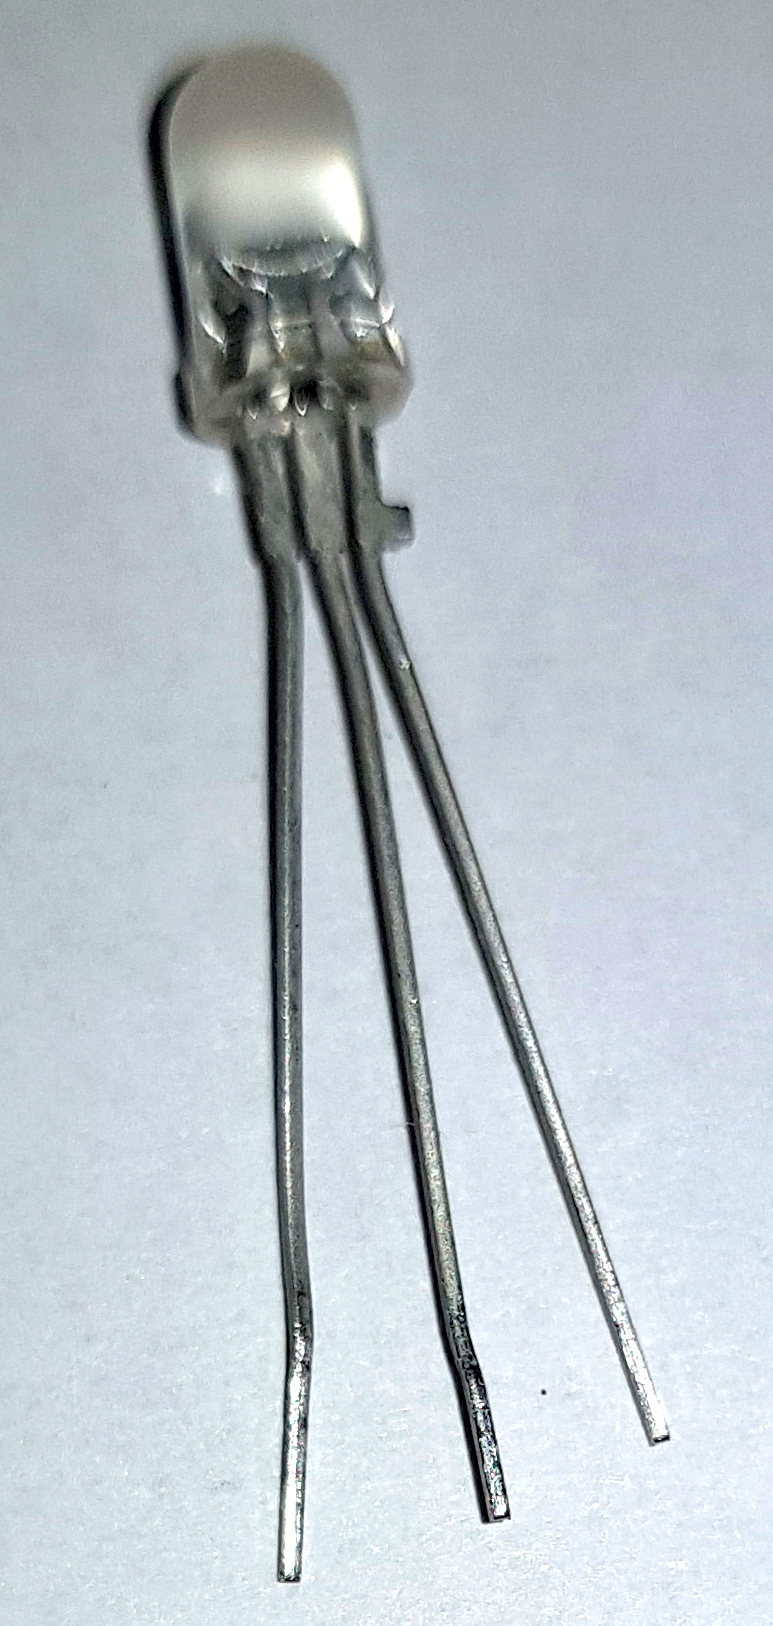
\includegraphics[width=0.7\textwidth,height=3.5cm]{figuren/dualled}
		\caption{een dual LED}
		\label{fig:dualLed}
	\end{subfigure}
	\hfill
	\begin{subfigure}[b]{0.3\textwidth}
		\centering
		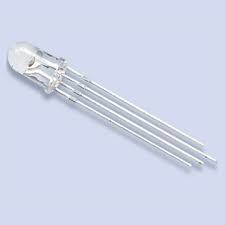
\includegraphics[width=0.9\textwidth,height=3.5cm]{figuren/rgbled}
		\caption{een RGB LED}
		\label{fig:rgbLed}
	\end{subfigure}
	\caption{Verschillende type LEDs}
	\label{fig:LEDs}
\end{figure}

De analist die de eisen voor de controller-software voor de LED controllers opstelt, heeft bedacht dat het in de toekomst mogelijk moet kunnen zijn om nieuwe LED types toe te voegen, bijvoorbeeld 3 kleuren LEDS. De controller software moet dus zo veel mogelijk onafhankelijk van het concrete LED type gemaakt worden. In figuur \ref{fig:klassLed} wordt de UML weergave geaan van zowel de SingleLed als de RGBLed
\begin{figure}[h!]
	\captionsetup{justification=centering}
	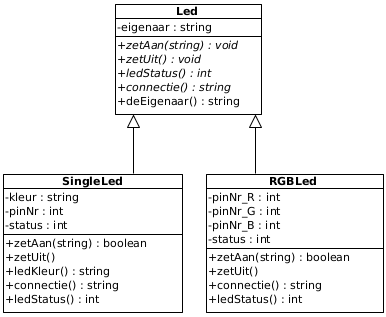
\includegraphics[width=0.6 \linewidth]{figuren/rgbKlasse}
	\centering
	\caption{De afgeleide klassen singleLed en RGBLed .}
	\label{fig:klasAfg}
\end{figure}
\newpage
De werking is als volgt.

\begin{itemize}
	\item Een LED wordt aangezet door de methode bool zetAan(string k); waarbij de parameter de kleur is die aangezet moet worden.
	\begin{itemize}
		\item Wordt bij een groene LED ''groen''  meegegeven, wordt de LED aangezet en true geretourneerd.
		\item Wordt bij een groene LED ''rood'' meegegeven, wordt de LED niet aangezet en wordt false geretourneerd.
	\end{itemize}
\item Een LED wordt uitgezet door de methode void zetUit(); Dit houd in dat bij een RGBLed alle kleuren uitgezet worden.
\item De methode string connectie(); geeft het gpioNummer van het aangesloten platform mee terug. In het geval van de RGBLed wordt een string mee teruggegeven met alle drie de gpioNummers gescheiden door een spatie.
\item Doordat de status van de LED verschillend zijn (een singleLed kan alleen aan en uit terwijl bij de RGBLed kan kleur1, kleur 2, kleur 3 of een combinatie van kleuren aan- en uitgaan), heeft elke afgeleide LED een eigen status.
	
\end{itemize}

\paragraph{Opdracht} 


